\documentclass[a4paper]{article}
\usepackage{times}
\usepackage[utf8]{inputenc}
\usepackage{selinput}
\usepackage{upquote}
\usepackage[margin=2cm, rmargin=4cm, tmargin=3cm]{geometry}
\usepackage{tcolorbox}
\usepackage{xspace}
\usepackage[french]{babel}
\usepackage{url}
\usepackage{hyperref}
\usepackage{fontawesome5}
\usepackage{marginnote}
\usepackage{ulem}
\usepackage{tcolorbox}
\usepackage{graphicx}
%\usepackage[top=Bcm, bottom=Hcm, outer=Ccm, inner=Acm, heightrounded, marginparwidth=Ecm, marginparsep=Dcm]{geometry}


\newtcolorbox{Example}[1]{colback=white,left=20pt,colframe=slideblue,fonttitle=\bfseries,title=#1}
\newtcolorbox{Solutions}[1]{colback=white,left=20pt,colframe=green,fonttitle=\bfseries,title=#1}
\newtcolorbox{Conseils}[1]{colback=white,left=20pt,colframe=slideblue,fonttitle=\bfseries,title=#1}
\newtcolorbox{Warning}[1]{colback=white,left=20pt,colframe=warning,fonttitle=\bfseries,title=#1}

\setlength\parindent{0pt}

  %Exercice environment
  \newcounter{exercice}
  \newenvironment{Exercice}[1][]
  {
  \par
  \stepcounter{exercice}\textbf{Question \arabic{exercice}:} (\faClock \enskip \textit{#1})
  }
  {\bigskip}
  

% Title
\newcommand{\titre}{\begin{center}
  \section*{Algorithmes et Pensée Computationnelle}
\end{center}}
\newcommand{\cours}[1]
{\begin{center} 
  \textit{#1}\\
\end{center}
  }


\newcommand{\exemple}[1]{\newline~\textbf{Exemple :} #1}
%\newcommand{\attention}[1]{\newline\faExclamationTriangle~\textbf{Attention :} #1}

% Documentation url (escape \# in the TP document)
\newcommand{\documentation}[1]{\faBookOpen~Documentation : \href{#1}{#1}}

% Clef API
\newcommand{\apikey}[1]{\faKey~Clé API : \lstinline{#1}}
\newcommand{\apiendpoint}[1]{\faGlobe~Url de base de l'API \href{#1}{#1}}

%Listing Python style
\usepackage{color}
\definecolor{slideblue}{RGB}{33,131,189}
\definecolor{green}{RGB}{0,190,100}
\definecolor{blue}{RGB}{121,142,213}
\definecolor{grey}{RGB}{120,120,120}
\definecolor{warning}{RGB}{235,186,1}

\usepackage{listings}
\lstdefinelanguage{texte}{
    keywordstyle=\color{black},
    numbers=none,
    frame=none,
    literate=
           {é}{{\'e}}1
           {è}{{\`e}}1
           {ê}{{\^e}}1
           {à}{{\`a}}1
           {â}{{\^a}}1
           {ù}{{\`u}}1
           {ü}{{\"u}}1
           {î}{{\^i}}1
           {ï}{{\"i}}1
           {ë}{{\"e}}1
           {Ç}{{\,C}}1
           {ç}{{\,c}}1,
    columns=fullflexible,keepspaces,
	breaklines=true,
	breakatwhitespace=true,
}
\lstset{
    language=Python,
	basicstyle=\bfseries\footnotesize,
	breaklines=true,
	breakatwhitespace=true,
	commentstyle=\color{grey},
	stringstyle=\color{slideblue},
  keywordstyle=\color{slideblue},
	morekeywords={with, as, True, False, Float, join, None, main, argparse, self, sort, __eq__, __add__, __ne__, __radd__, __del__, __ge__, __gt__, split, os, endswith, is_file, scandir, @classmethod},
	deletekeywords={id},
	showspaces=false,
	showstringspaces=false,
	columns=fullflexible,keepspaces,
	literate=
           {é}{{\'e}}1
           {è}{{\`e}}1
           {ê}{{\^e}}1
           {à}{{\`a}}1
           {â}{{\^a}}1
           {ù}{{\`u}}1
           {ü}{{\"u}}1
           {î}{{\^i}}1
           {ï}{{\"i}}1
           {ë}{{\"e}}1
           {Ç}{{\,C}}1
           {ç}{{\,c}}1,
    numbers=left,
}

\newtcbox{\mybox}{nobeforeafter,colframe=white,colback=slideblue,boxrule=0.5pt,arc=1.5pt, boxsep=0pt,left=2pt,right=2pt,top=2pt,bottom=2pt,tcbox raise base}
\newcommand{\projet}{\mybox{\textcolor{white}{\small projet}}\xspace}
\newcommand{\optionnel}{\mybox{\textcolor{white}{\small Optionnel}}\xspace}
\newcommand{\advanced}{\mybox{\textcolor{white}{\small Pour aller plus loin}}\xspace}
\newcommand{\auto}{\mybox{\textcolor{white}{\small Auto-évaluation}}\xspace}


\usepackage{environ}
\newif\ifShowSolution
\NewEnviron{solution}{
  \ifShowSolution
	\begin{Solutions}{\faTerminal \enskip Solution}
		\BODY
	\end{Solutions}
  \fi}


  \usepackage{environ}
  \newif\ifShowConseil
  \NewEnviron{conseil}{
    \ifShowConseil
    \begin{Conseils}{\faLightbulb \quad Conseil}
      \BODY
    \end{Conseils}

    \fi}

    \usepackage{environ}
  \newif\ifShowWarning
  \NewEnviron{attention}{
    \ifShowWarning
    \begin{Warning}{\faExclamationTriangle \quad Attention}
      \BODY
    \end{Warning}

    \fi}
  

%\newcommand{\Conseil}[1]{\ifShowIndice\ \newline\faLightbulb[regular]~#1\fi}




\begin{document}

% Change the following values to true to show the solutions or/and the hints
\ShowSolutiontrue
\ShowConseiltrue
\titre
\cours{Complexité, Classes et Polymorphisme- exercices basiques}

Le but de cette série d'exercices est d'aborder les notions présentées durant la séance de cours. Cette série d'exercices sera orientée autour des points suivants:
\begin{enumerate}
    \item La complexité des algorithmes
    \item La programmation orientée objet 
    \item Le polymorphisme
\end{enumerate}

Les languages de programmation qui seront utilisés pour cette série d'exercices sont Java et Python.

Le temps indiqué (\faClock) est à titre indicatif.


\section{Complexité (40 minutes)}

Pour chacun des programmes ci-dessous, donnés à chaque fois en Python et Java, indiquez en une phrase, ce que font ces algorithmes et calculez leur complexité temporelle avec la notation $O( )$. Le code est écrit en Python et en Java. \\

\begin{Exercice}[10 minutes] \textbf{Complexité} \\

    Quelle est la complexité du programme ci-dessous?\\
    \textbf{Python :}
    \begin{lstlisting}{language=Python}
    # Entrée: n un nombre entier
    def algo1(n):
        s = 0
        for i in range(10*n):
            s += i
        return s
    \end{lstlisting}
    
    \textbf{Java :}
    \begin{lstlisting}{language=Java}
        public static int algo1(int n) {
            int s = 0;
            for (int i=0; i < 10*n; i++){
                s += i;
            }
            return s;
        }
    \end{lstlisting}

    \begin{enumerate}
        \item $O(n)$
        \item $O(n^3)$
        \item $O(\log(n))$
        \item $O(n^n)$
    \end{enumerate}
    
    \begin{conseil}
    Rappelez vous que la notation $O()$ sert à exprimer la complexité d'algorithmes dans le \textbf{pire des cas}. Les règles suivantes vous seront utiles. Pour $n$ étant la taille de vos données, on a que :
    \begin{enumerate}
        \item Les constantes sont ignorées : $O(2n) = 2*O(n) = O(n)$ 
        \item Les termes dominés sont ignorés : $O(2n^2+5n+50)$ = $O(n^2)$
    \end{enumerate}
    \end{conseil}

    \begin{solution}
        L'algorithme est composé d'une boucle qui incrémente une variable \lstinline{s}. Il effectue $10*n$ l'opération et par conséquent a une complexité de $O(n)$.
    \end{solution}
\end{Exercice}
\newpage
\begin{Exercice}[10 minutes] \textbf{Complexité} \\
    Quelle est la complexité du programme ci-dessous?\\
    \textbf{Python :}
    \begin{lstlisting}[language=Python]
        # Entrée: L est une liste de nombres entiers et M un nombre entier
        def algo2(L, M):
            i = 0
            while i < len(L) and L[i] <= M:
                i += 1
            s = i - 1
            return s
    \end{lstlisting}
    
    \textbf{Java :}
    \begin{lstlisting}[language=Java]
        public static int algo2(int[] L, int M) {
            int i = 0;
            while (i < L.length && L[i] <= M){
                i += 1;
            }
            int s = i - 1;
            return s;
        }
    \end{lstlisting}

    \begin{enumerate}
        \item $O(n^3)$
        \item $O(\log(n))$
        \item $O(n)$
        \item $O(n^n)$
    \end{enumerate}

    \begin{solution}
    L'algorithme est composé d'une boucle \lstinline{while} qui va parcourir une liste \lstinline{L} jusqu'à trouver une valeur qui est supérieure à \lstinline{M}. Ainsi, dans le pire des cas, l'algorithme parcourt toute la liste, et a donc une complexité de $O(n)$, $n$ étant la taille de la liste.
    \end{solution}
\end{Exercice}
\begin{Exercice}[10 minutes] \textbf{Complexité} \\
    Quelle est la complexité du programme ci-dessous?\\
        \textbf{Python :}
        \begin{lstlisting}[language=Python]
        #Entrée: L et M sont 2 listes de nombre entiers
        def algo3(L, M):
            n = len(L)
            m = len(M)
            for i in range(n):
                L[i] = L[i]*2
            for j in range(m):
                M[j] = M[j]%2
        \end{lstlisting}
        
        \textbf{Java :}
        \begin{lstlisting}[language=Java]
            public static void algo3(int[] L, int[] M) {
                int n = L.length;
                int m = M.length;
                for (int i=0; i < n; i++){
                    L[i] = L[i]*2;
                }
                for (int j=0; j < m; j++){
                    M[j] = M[j]%2;
                }
            }
        \end{lstlisting}

        \begin{enumerate}
            \item $O(n^2)$
            \item $O(n + m)$
            \item $O(n)$
            \item $O(2^n)$
        \end{enumerate}

        \begin{solution}
        L'algorithme est composé de 2 boucles. La première parcourt une liste \lstinline{L} et multiplie par 2 les éléments de la liste. 
        L'autre parcourt une liste \lstinline{M} et assigne à chaque élément le reste de la division euclidienne de l'élément par 2. 
        Soient $n$ et $m$ les tailles respectives de \lstinline{L} et de \lstinline{M}, on obtient une complexité de $O(n + m)$. 
        Ainsi, l'élément ayant la plus grande complexité sera utilisé pour déterminer la complexité de l'algorithme dans son ensemble.
        \end{solution}
\end{Exercice}

\begin{Exercice}[10 minutes] \textbf{Complexité} \\
    Quelle est la complexité du programme ci-dessous?\\
    \textbf{Python :}
    \begin{lstlisting}[language=Python]
    #Entrée: L est une liste de nombre entiers
    def algo4(L):
        n = len(L)
        i = 0
        s = 0
        while i < math.log(n):
            s += L[i]
            i += 1
        return s
    \end{lstlisting}
    
    \textbf{Java :}
    \begin{lstlisting}[language=Java]
        import java.lang.Math; 

        public static void algo4(int[] L) {
            int n = L.length;
            int s = 0;
            for (int i=0; i < Math.log(n); i++){
                s += L[i];
            }
        }
    \end{lstlisting}

    \begin{enumerate}
        \item $O(n^2)$
        \item $O(n)$
        \item $O(\log(n))$
        \item $O(n^n)$
    \end{enumerate}

    \begin{solution}
    L'algorithme est composé d'une boucle qui va itérer sur $\log(n)$ éléments et 
    va calculer la somme de ces éléments. Ainsi, l'algorithme a une complexité de $O(\log n)$.
    Le temps d'exécution de ce programme peut être visualisé sur la courbe jaune du graphe ci-dessous (\ref{bigO}).
    \end{solution}
    
    \begin{figure}[h!]
        \centering
        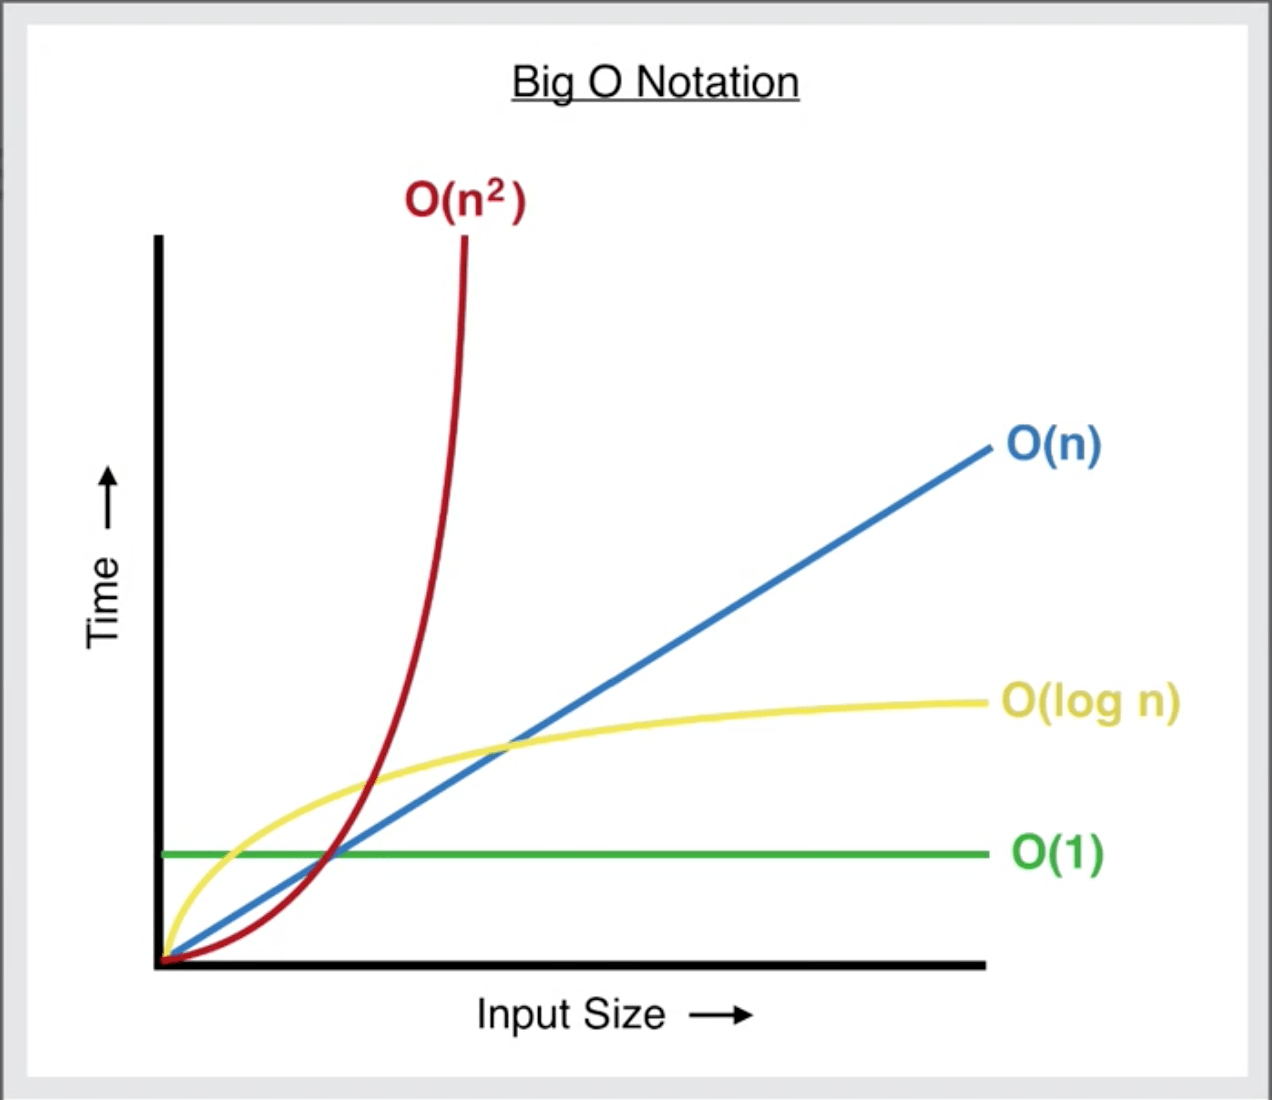
\includegraphics[width=10cm]{ressources/complexity.png}
        \caption{Représentation de complexités temporelles}
        \label{bigO}
    \end{figure}

    

\end{Exercice}
\newpage

\section{Création de votre première classe en Java (30 minutes)}

Le but de cette première partie est de créer votre propre classe en Java. Cette classe sera une classe nommée \lstinline{Dog()} représentant un chien. Elle aura plusieurs attributs et méthodes que vous implémenterez au fur et à mesure.
\\

\begin{Exercice}[10 minutes] Création de classe et encapsulation\\
    Commencez par créer une nouvelle classe \lstinline{Dog} dans votre projet. Ensuite, créez les attributs suivants :
    \begin{enumerate}
    \item Un attribut \lstinline{public} String nommé \lstinline{name}
    \item Un attribut \lstinline{private} List nommé \lstinline{tricks}
    \item Un attribut \lstinline{private} String nommé \lstinline{race}
    \item Un attribut \lstinline{private} int nommé \lstinline{age}
    \item Un attribut \lstinline{private} int nommé \lstinline{mood} initialisé à 5 (correspondant à l'humeur du chien)
    \item Un attribut de classe (\lstinline{static}) \lstinline{private} int nommé \lstinline{nb_chiens}
   	\end{enumerate}
   	
   	Créez une méthode publique du même nom que la classe (\lstinline{Dog}). Cette méthode est appelée le \lstinline{constructeur}, elle va servir à initialiser les différentes instances de notre classe. Un \lstinline{constructeur} en \lstinline{Java} aura le même nom que la classe, et le \lstinline{constructeur} en \lstinline{Python} sera défini par la méthode \lstinline{__init__}. Cette méthode prendra en argument les éléments suivants qui seront utilisés pour initialiser les attributs de notre instance :
   	\begin{enumerate}
    \item Une chaîne de caractère \lstinline{name},
    \item Une liste \lstinline{tricks},
    \item Une chaîne de caractère \lstinline{race},
    \item Un entier \lstinline{age}.
   	\end{enumerate}
   	
   	Pour finir, cette méthode doit incrémenter l'attribut de classe \lstinline{nb_chiens} qui va garder en mémoire le nombre d'instances crées.
   	
\begin{conseil}
    %Modifier le conseil
    Pour revoir les notions de base du langage Java, n'hésitez pas à consulter le guide de démarrage en Java sur Moodle:
	\url{https://moodle.unil.ch/mod/folder/view.php?id=1132337}

   Pour cet exercice, n'oubliez pas de préciser si vos attributs sont \lstinline{public} ou \lstinline{private}.
   
   Le mot \lstinline{static} correspond à un élément de classe (attribut ou méthode), cet élément pourra ensuite être appelé via la classe directement.
   
   Pour attribuer des valeurs à vos attributs d'instance, utilisez le mot-clé \lstinline{this.attribut}.
   
   Pour accéder aux attributs de classe, utilisez \lstinline{nom_classe.nom_attribut}
\end{conseil}
    
\begin{solution}
	\lstinputlisting{solutions/Question1.java}
\end{solution}
\end{Exercice}

\begin{Exercice}[10 minutes] Getters et setters\\
    Il faut maintenant créer des méthodes de type \lstinline{getter} et \lstinline{setter} afin d'interagir avec les attributs \lstinline{private} des instances de la classe. 
    Les \lstinline{getters} renverront les attributs souhaités tandis que les \lstinline{setters} les modifieront.

    Les \lstinline{setters} sont souvent utilisés pour modifier la valeur d'attributs privés et ne renvoient rien.
    \begin{conseil}
        Exemple de \lstinline{getters} et de \lstinline{setters}:
        \lstinputlisting{ressources/Example.java}
    \end{conseil} 

    Vous pouvez directement accéder à des attributs publics en utilisant \lstinline{nom_instance.attribut} à l'intérieur ou à l'extérieur de la classe. \\
    
    Créez les méthodes suivantes :
    \begin{itemize}
    \item \lstinline{getTricks()}
    \item \lstinline{getRace()}
    \item \lstinline{getAge()}
    \item \lstinline{getMood()}
    \item \lstinline{setTricks()}
    \item \lstinline{setRace()}
    \item \lstinline{setAge()}
    \item \lstinline{setMood()}
    \end{itemize}
    
    Créez également une méthode de classe permettant de retourner le nombre de \lstinline{Dog} instanciés (un \lstinline{getter}).
   	
\begin{conseil}
    Intellij vous permet de générer automatiquement certaines méthodes telles que les getters et setters. Vous pouvez consulter le lien suivant pour plus d'informations: \url{https://www.jetbrains.com/help/idea/generating-code.html\#generate-delegation-methods}.
    \\
    Toutefois, pour cet exercice, nous vous encourageons à le faire manuellement.
\end{conseil}
    
\begin{solution}
	\lstinputlisting{solutions/Question2.java}
\end{solution}
\end{Exercice}


\begin{Exercice}[5 minutes] Manipulation d'attributs - Listes\\
    Créez une méthode publique nommée \lstinline{addTrick(String trick)} qui prend en entrée une chaîne de caractères et l'ajoute à la liste \lstinline{tricks}. \\
   	
\begin{conseil}
   La liste \lstinline{tricks} est une liste comme les autres. Si vous voulez la modifier, vous aurez besoin de passer par une \lstinline{LinkedList} temporaire.
\end{conseil}
    
\begin{solution}
	\lstinputlisting{solutions/Question3.java}
\end{solution}
\end{Exercice}

\begin{Exercice}[5 minutes] Manipulation d'attributs - \lstinline{setter}\\
    Créez deux méthodes permettant de modifier l'attribut \lstinline{mood} de l'objet \lstinline{Dog}. La méthode \lstinline{leash()} décrémentera \lstinline{mood} de 1 et \lstinline{eat()} l'incrémentera de 3. \\

\begin{solution}
	\lstinputlisting{solutions/Question4.java}
\end{solution}
\end{Exercice}

\begin{Exercice}[5 minutes] Manipulation d'attributs d'une autre instance\\
    Créez une méthode nommée \lstinline{getOldest (Dog other)} qui prend comme argument un élément de type \lstinline{Dog}, puis retourne le nom et l'âge du chien le plus agé sous le format suivant : ``\lstinline{nomChien} est le chien le plus agé avec \lstinline{ageChien} ans''. \\
   	
\begin{conseil}
   L'élément \lstinline{Dog} que vous passez en argument est un objet de type \lstinline{Dog}, vous pouvez donc lui appliquer les méthodes que vous avez créé tout à l'heure.
   Faites attention à la façon d'accéder aux différents attributs de votre deuxième chien (pour rappel, les attributs privés ne sont accessibles qu'à travers des \lstinline{getters} que vous aurez préalablement définis).
\end{conseil}
    
\begin{solution}
	\lstinputlisting{solutions/Question5.java}
\end{solution}
\end{Exercice}

\begin{Exercice}[5 minutes] Redéfinition de méthodes\\
    Créez une méthode \lstinline{toString()} de type \lstinline{public} qui retourne une chaîne de caractères contenant toutes les informations d'une instance de \lstinline{Dog}. Ainsi, dans votre \lstinline{main}, en faisant \lstinline{System.out.println(...)} sur une instance de \lstinline{Dog}, vous obtiendrez un texte sous le format suivant: 
    ``\lstinline{nomChien} a \lstinline{ageChien} ans, est un \lstinline{raceChien} et a une humeur de \lstinline{moodChien}. Il sait faire les tours suivants : \lstinline{tricksChien}''.
    \begin{Example}{\faLightbulb \quad Informations utiles}
        La méthode \lstinline{toString()} hérite de la super classe \lstinline{Object}. La notion d'héritage sera présentée la semaine prochaine. Retenez juste qu'il est possible de choisir ce que vaudra le texte descriptif de nos objets de type \lstinline{Dog}. Il est également possible de redéfinir d'autres méthodes comme par exemple l'addition ou la soustraction, ce qui permettrait de choisir comment 2 objets de type \lstinline{Dog} seraient additionnés ou soustraits.
        Avant de redéfinir la méthode \lstinline{toString()}, ajoutez l'annotation \lstinline{@Override}.
        \\
    \end{Example}
    \begin{solution}
        \lstinputlisting{solutions/Question6.java}
    \end{solution}
\end{Exercice}
Pour contrôler que vos méthodes et attributs ont été implémentés correctement, vous pouvez essayer le code suivant à l'intérieur de votre méthode \lstinline{main} :
	\lstinputlisting{ressources/question6_main.java}
	
Vous devriez obtenir ce résultat :
    \lstinputlisting{ressources/mainsolution.java}


\newpage
\section{Notions de POO en Python (30 minutes)}
Dans cette section, nous créerons pas-à-pas une classe \lstinline{Point} contenant des attributs et des méthodes utiles.
Dans votre IDE, créez un nouveau projet Python (Fichier $>$ Nouveau $>$ Projet). Dans un dossier de votre choix, créez un fichier \lstinline{question11.py}.\\
\begin{Exercice}[15 minutes] Classe \lstinline{Point}
    \begin{itemize}
        \item Créez une classe \lstinline{Point} et un constructeur par défaut contenant deux paramètres (\lstinline{x} et \lstinline{y}).
        \begin{conseil}
            Pour rappel, un constructeur est une fonction \lstinline{__init()__} que vous redéfinirez dans votre classe.
        \end{conseil}
        \item Définissez deux attributs privés pour votre classe \lstinline{Point}. Ces attributs seront les coordonnées x et y de vos points. Par défaut, assignez leur les valeurs données dans le constructeur.
        \begin{conseil}
            À l'intérieur d'une classe, utilisez le mot-clé \lstinline{self} pour accéder aux méthodes et attributs de l'instance que vous manipulez.
            En Python, pour spécifier qu'un attribut est privé, rajouter un double underscore au nom de l'attribut (Exemple: \lstinline{__score=0})
        \end{conseil}
        \item Définir des getters et setters.
        \begin{conseil}
            En Python, le mot-clé \lstinline{self} est l'équivalent de \lstinline{this} utilisé en Java.
        \end{conseil}
        \item Définissez une méthode \lstinline{distance} qui prend en entrée l'instance du \lstinline{Point} (\lstinline{self}) et un autre \lstinline{Point} \lstinline{p2}. Cette méthode \lstinline{distance} retournera la distance euclidienne entre le point \lstinline{self} et \lstinline{p2}. 
        \begin{conseil}
            Pour rappel, la distance euclidienne entre deux points est définie par la formule $\sqrt{(x_1 - x_2)^2 + (y_1 - y_2)^2}$.
            Utilisez la fonction \lstinline{sqrt()} de la librairie \lstinline{math} pour calculer la racine carrée. Pensez à importer la libraire \lstinline{math}.
        \end{conseil}
        \item Définissez une méthode \lstinline{milieu} qui prendra en entrée \lstinline{self} et \lstinline{p2} et qui retournera un objet \lstinline{Point} situé entre \lstinline{self} et \lstinline{p2}.
        \begin{conseil}
            Pour trouver les coordonnées d'un point M($x_M$, $y_M$) situé au milieu du segment défini par des points A($x_A$, $y_A$) et B($x_B, y_B$),
            utilisez les formules suivantes:
            $x_M = \frac{x_1 + x_2}{2}$ et $y_M = \frac{y_1 + y_2}{2}$
        \end{conseil}
        \item Redéfinissez une méthode \lstinline{__str__()} dans la classe \lstinline{Point} qui retournera une chaîne de caractères contenant les coordonnées $(x,y)$ d'un point. Ainsi, lorsqu'on fera un \lstinline{print} d'une instance de la classe \lstinline{Point}, le message qui s'affichera sera le suivant:
        \textit{Les coordonnées du Point sont: x = "remplacez par la valeur de x" et y = "remplacez par la valeur de y"}
    \end{itemize}
\end{Exercice}
\begin{solution}
    \lstinputlisting{solutions/question11_solution.py}
\end{solution}

\newpage

\section{Notions d'héritage - Java (30 minutes)}

Le but de cette partie est de mettre en pratique les notions liées à l'héritage. 
Nous allons créer une classe \lstinline{Livre()} qui représentera notre classe-mère. Nous allons également créer deux classes filles, \lstinline{Livre_Audio()} et \lstinline{Livre_Illustre()}. Les classes filles hériteront des attributs et méthodes de la classe-mère. \\

\begin{Exercice}[20 minutes] \lstinline{Création des différentes classes}\\
Créez la classe-mère \lstinline{Livre} avec les caractéristiques suivantes:
\begin{itemize}
	\item un attribut \lstinline{privé String} nommé \lstinline{titre},
	\item un attribut \lstinline{privé String} nommé \lstinline{auteur},
	\item un attribut \lstinline{privé int} nommé \lstinline{annee},
	\item un attribut \lstinline{privé int} nommé \lstinline{note} (initialisé à \lstinline{-1}),
	\item le \lstinline{constructeur} de la classe qui prendra les trois premiers arguments cités ci-dessus,
	\item une méthode \lstinline{setNote()} qui permet de définir l'attribut \lstinline{note},
	\item une méthode \lstinline{getNote()} qui permet de retourner l'attribut \lstinline{note},
	\item une méthode \lstinline{toString()} qui retournera le titre, l'auteur, l'année et la note d'un ouvrage \lstinline{note} (réécrire cette méthode permettra d'afficher un objet \lstinline{Livre} en utilisant \lstinline{System.out.println()}). \\
\end{itemize}

Attention, si la \lstinline{note} n'a pas été modifiée et qu'elle vaut toujours \lstinline{-1}, affichez ``Note : pas encore attribuée'' au lieu de ``Note : \lstinline{note}'' via la méthode \lstinline{toString()}. \\
Créez les classes filles avec les caractéristiques suivantes:\\
\lstinline{class Livre_Audio extends Livre}
\begin{itemize}
	\item un attribut \lstinline{privé String} nommé \lstinline{narrateur}
\end{itemize}
\lstinline{class Livre_Illustre extends Livre}
\begin{itemize}
	\item un attribut \lstinline{privé String} nommé \lstinline{illustrateur}
\end{itemize}
Voici le squelette du programme à compléter:
\begin{lstlisting}
	class Livre {
	}
	class Livre_Audio extends Livre {
	}
	class Livre_Illustre extends Livre {
	}\end{lstlisting}
\begin{conseil}
En Java, lors de la déclaration d'une classe, le mot clé \lstinline{extends} permet d'indiquer qu'il s'agit d'une classe fille de la classe indiquée. 
Le mot clé \lstinline{super} permet à la sous classe d'hériter d'éléments de la classe-mère. \lstinline{super} peut être utilisé dans le constructeur de la classe-fill selon l'example suivant: \lstinline{super(attribut_mère_1, attribut_mère_2, attribut_mère_3, etc.);}. Ainsi, il n'est pas nécessaire de redéfinir tous les attributs d'une classe fille !
L'instruction \lstinline{super} doit toujours être la première instruction dans le constructeur d'une classe-fille.
Vous pouvez vous servir de \lstinline{'\\n'} dans une chaîne de caractères pour effectuer un retour à la ligne lors de l'affichage d'une chaîne de caractères.
\end{conseil}
\begin{solution}
	\lstinputlisting{solutions/heritage-solution-1.java}
\end{solution}
\end{Exercice}
\begin{Exercice}[5 minutes] \lstinline{Méthode et héritage} \\
Maintenant que vous avez créé la classe-mère et les classes filles correspondantes, vous pouvez créer un objet \lstinline{Livre} à l'aide du constructeur de la classe \lstinline{Livre_Audio} (et des arguments donnés lors de la création de l'objet).
% TODO: Phrase à reformuler. S'agit-il de valeurs par défaut du constructeur ou des valeurs de l'instance?
En instanciant l'objet, vous pourriez utiliser les valeurs suivantes :\\
titre: ``Hamlet'', auteur: ``Shakespeare'', année: ``1609'' et le narrateur ``William''.\\
Une fois l'objet créé, attribuez-lui une note à l'aide de la méthode \lstinline{setNote()} définie précédemment.\\ 
Finalement, utilisez la méthode \lstinline{System.out.println()} pour afficher les informations du livre.\\
Redéfinir la méthode \lstinline{toString()} de la classe \lstinline{Livre_Audio} afin que la valeur de l'attribut \lstinline{narrateur} soit affichée.
Faites pareil avec la classe \lstinline{Livre_Illustre} et son attribut \lstinline{Illustrateur}
\begin{conseil}
\textbf{Attention}, vous devez créer un objet \lstinline{Livre} et non \lstinline{Livre_Audio}.
Le mot-clé \lstinline{super} peut être utilisé dans la redéfinition d'une méthode selon l'exemple suivant: \lstinline{super.nom_de_la_methode();}. Le mot clé \lstinline{super} représente la classe parent, tout comme le mot clé \lstinline{this} fait référence à l'instance avec laquelle la méthode est appelée. 
L'instruction \lstinline{super} doit toujours être la première instruction dans le redéfinition d'une méthode dans une classe fille. 
\end{conseil}
\begin{solution}
	\lstinputlisting{solutions/heritage-solution-2.java}
	\lstinputlisting{solutions/heritage-solution-3.java}
\end{solution}
\end{Exercice}
\newpage
Lorsque toutes les étapes auront été effectuées, placez le code suivant dans votre \lstinline{main} et exécutez votre programme:\\
\lstinputlisting{ressources/heritage-main.java}
Vous devriez obtenir : \\
\lstinputlisting{ressources/heritage-main-prompt.java}


\end{document}
